\documentclass[10pt]{article}
\usepackage[margin=0.75in]{geometry}
\usepackage{graphicx,mathptmx}
\usepackage[hidelinks]{hyperref}
\title{Exact primality and functional witness optimization}
\author{Native implementation and validation receipt}
\date{30 October 2026}
\begin{document}
\maketitle
\noindent\textbf{Code and bounded correctness checks complete; performance measurements blocked.}
Both published challenge scalars remain unresolved. These are native engineering
changes; no runtime, end-to-end or asymptotic speedup is claimed.
\begin{center}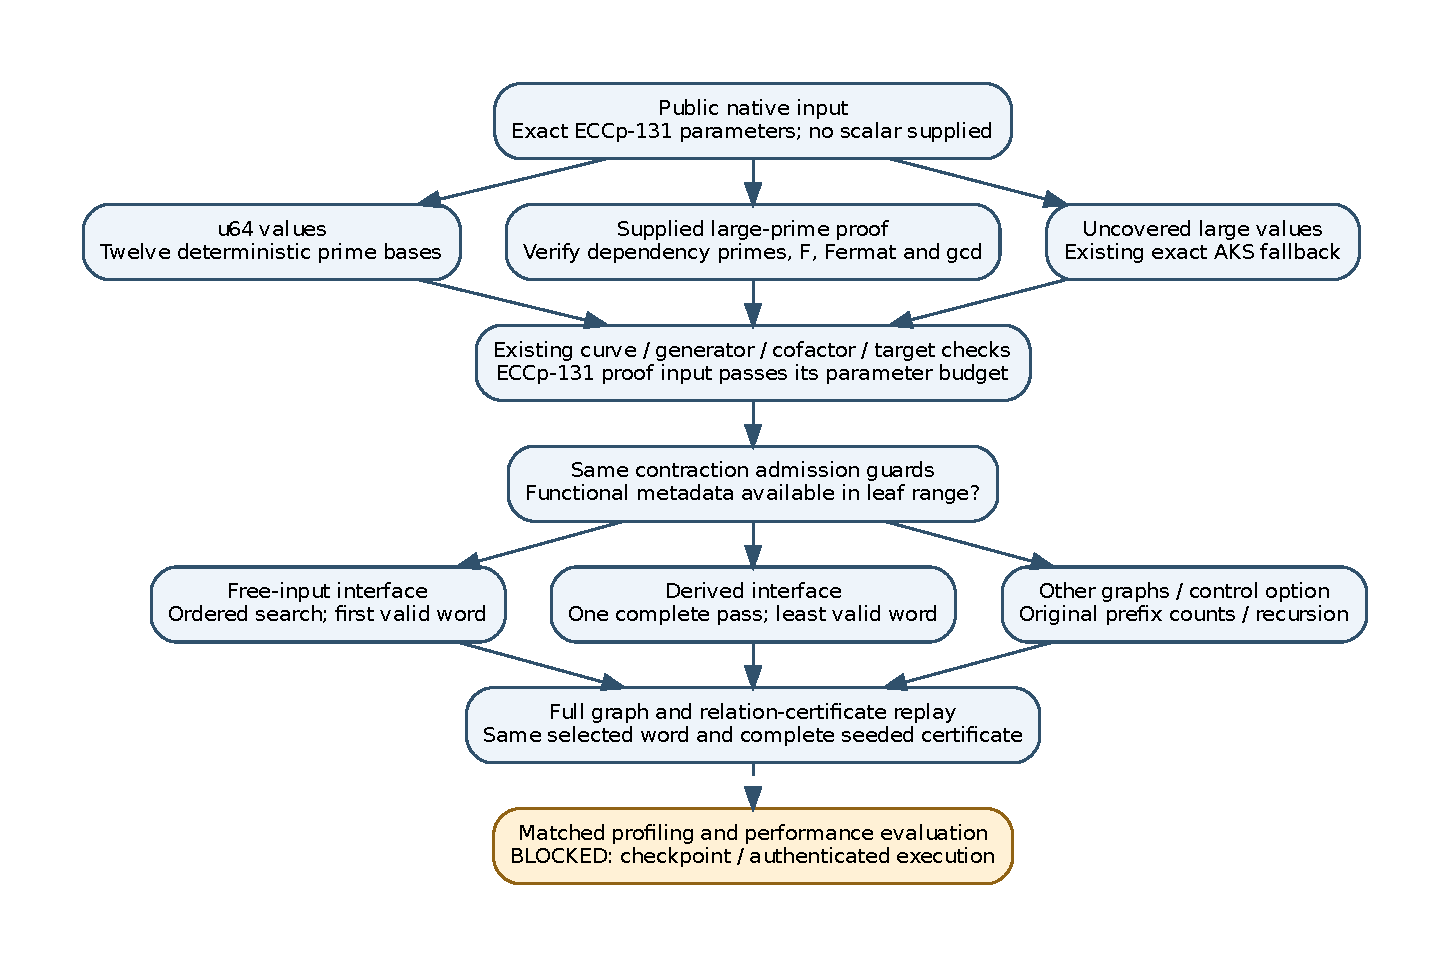
\includegraphics[width=\linewidth,height=5.2in,keepaspectratio]{paths.pdf}\end{center}
\noindent Solid paths are implemented and tested. The dashed path is an open
measurement requirement; no profile or scientific benchmark was launched after
the S3 checkpoint gate failed.
\newpage
\section*{Observed correctness}
The native suite passes 34 tests, including an identical complete seeded
relation certificate under the original prefix-count path and optimized search.
Strict lint and declared Rust 1.78 checks pass. Prime controls compare values
through 100,000 with an independent sieve and reject forged proof nodes;
witness controls cover derived interfaces, ordering, pins, aliases, UNSAT and
resource exhaustion. The certified ECCp-131 input passes parameter/target
validation at 5,589 uncalibrated charged steps within its original two-million
step policy. It supplies no secret scalar and does not establish relation-search
feasibility or a complete challenge solve.
\begin{center}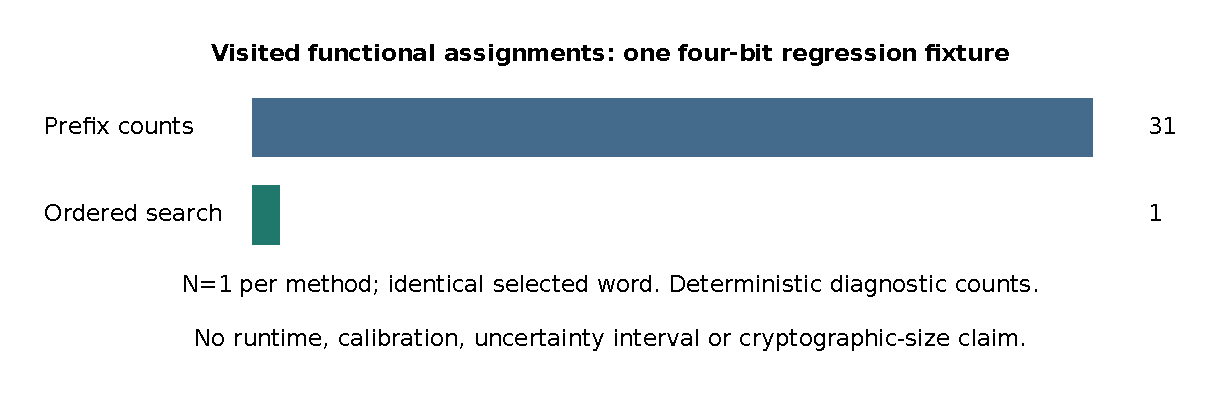
\includegraphics[width=\linewidth]{witness-work.pdf}\end{center}
\noindent The plot reports one deterministic regression case per method, not a
runtime or cryptographic-size result. Exact count behavior and source recursion
guards are unchanged. A free-input interface is searched in its interface order;
a derived interface requires a full pass and minimum selection. Every returned
assignment still passes graph evaluation. The original path is selectable.
\section*{Limits and evidence}
Proof-fixture preparation cost is unpriced. Baseline/candidate calibrated
operation totals, S/rho, A/A, matched A/B and runtime intervals remain absent.
The profiler probe lacked gawk and the checkpoint gate lacked an upload
transport; local unisolated test times are not benchmark evidence. The frozen
protocol retains the full requested comparison and fresh holdouts. No smaller
diagnostic discharges that requirement. Earlier compile/assertion failures and
their corrections are preserved in the raw development logs.

Sources: Handbook of Applied Cryptography, Fact 4.40 and chapter notes
(checked Pocklington proofs); Sorenson/Webster, arXiv:1509.00864 (the twelve-base
bound, restricted here to u64); the existing native/pinned contraction sources.
No new theorem, formal proof, practical subexponential result or leaderboard
promotion is claimed. The independent general audit remains open.
\end{document}
